\documentclass{article}

% if you need to pass options to natbib, use, e.g.:
% \PassOptionsToPackage{numbers, compress}{natbib}
% before loading nips_2017
%
% to avoid loading the natbib package, add option nonatbib:
% \usepackage[nonatbib]{nips_2017}

\usepackage[final]{nips_2017}

% to compile a camera-ready version, add the [final] option, e.g.:
% \usepackage[final]{nips_2017}

\usepackage[utf8]{inputenc} % allow utf-8 input
\usepackage[T1]{fontenc}    % use 8-bit T1 fonts
\usepackage{hyperref}       % hyperlinks
\usepackage{url}            % simple URL typesetting
\usepackage{booktabs}       % professional-quality tables
\usepackage{amsfonts}       % blackboard math symbols
\usepackage{nicefrac}       % compact symbols for 1/2, etc.
\usepackage{microtype}      % microtypography
\usepackage{graphicx}
\graphicspath{ {images/} }

\title{Nerual Phytolith Classifier}

% The \author macro works with any number of authors. There are two
% commands used to separate the names and addresses of multiple
% authors: \And and \AND.
%
% Using \And between authors leaves it to LaTeX to determine where to
% break the lines. Using \AND forces a line break at that point. So,
% if LaTeX puts 3 of 4 authors names on the first line, and the last
% on the second line, try using \AND instead of \And before the third
% author name.

\author{
  James Noeckel, Chenglong Wang\\
  University of Washington
}

\begin{document}
% \nipsfinalcopy is no longer used

\maketitle

\begin{abstract}
  We study the classification problem of phytoliths using stacks of images generated by scanning confocal microscopy. In this report, we present our methods of data preprocessing and dataset augmentation, as well as the accuracy of various models when used as classifiers. Due to the small volume of training data, we avoid using complex models, comparing the accuracy of a linear classifier, a neural network with one hidden fully-connected layer, a neural network with one hidden convolutional layer, and a neural network with two convolutional layers and three fully-connected layers. Additionally, we supervise the classifiers on all three labels (sub-family, tribe, and genus) during training, and additional training data is generated from existing data subjected to random transformations. The results show high performance in differentiating sub-families, and lower performance at the lower rungs of the hierarchy, where some labels have but one example. The single convolutional network performing best on genus and the two-convolutional and three-fully-connected network performing best on sub-family and tribe. The small amount of data makes interpreting test performance difficult, and our tree-based supervision or dataset augmentation do not have consistent effects on accuracy.
\end{abstract}

\section{Introduction}


Phytoliths are microscopic formations of silica found in plant tissues. Their persistence, along with the variation in their shapes and sizes make them particularly useful in archaeological and paleoenvironmental research. Consequently, there is interest in automatically classifying phytoliths from images. Phytolith formations are divided into sub-families, which are in turn divided into tribes, which consist of individual genera.

While there exists a variety of practical image classifiers, the problem for classifying confocal micrographs presents a number of challenges. Many real world objects, such as phytolith structures or medical scans, are represented in the form of 3D volumes. Instead of directly flattening 2D image stacks into a single image before feeding into a neural network, prior work shows that incorporating 3D structures in image embedding can significantly improve classification results.  In our case, there clearly exist structures that are most prevalent at specific depths, so that aggregating the layers seems like a poor choice. We therefore maintain three-dimensional images in the hopes that our classifiers can learn more meaningful features.

The dataset we used was fairly small (883 image stacks) for training and testing, given that this is an image classification problem. We made some attempts to rectify this using synthetic data samples generated from existing ones, by applying random rotations and scales. Also to aid in classification, we supervised the training using all of the hierarchical class labels together. We conducted a set of experiments using a linear classifier as a baseline, together with several neural net architectures, testing their performance on the dataset when classifying genus, tribe, and sub-family. Our results yield about 60\% accuracy on genus, the lowest level of classification, and about 95\% accuracy at differentiating between the two sub-families.

\section{Problem Description}

The raw data that we are considering for learning phytolith species consists of image stacks from confocal micrographs of individual specimen. The images have varying resolution, number of slices, average intensity levels and apparent lighting conditions. Considered as a whole, these image stacks encode a three-dimensional representation of the organisms. However, because each pixel is the result of focusing a cone of light at a particular point in the volume, each slice contains out-of-focus features from every other slice. This makes reconstructing an actual three-dimensional form or surface from the content of the 2D image slices is nontrivial.

The labels are hierarchical, consisting of subfamilies, tribes, and finally the species. All in all, there are 889 data points with around 20 examples per species. Although the data is incredibly high dimensional (in the tens of millions of dimensions) due to being volumetric, there are relatively few examples from which to learn. It is for this reason that we attempt to learn from features that may be present in the volumetric representation of the confocal micrograph, whether or not it corresponds well to the original geometry, in order to train a classifier to predict class labels from image stacks.

\begin{figure}
	\centering
		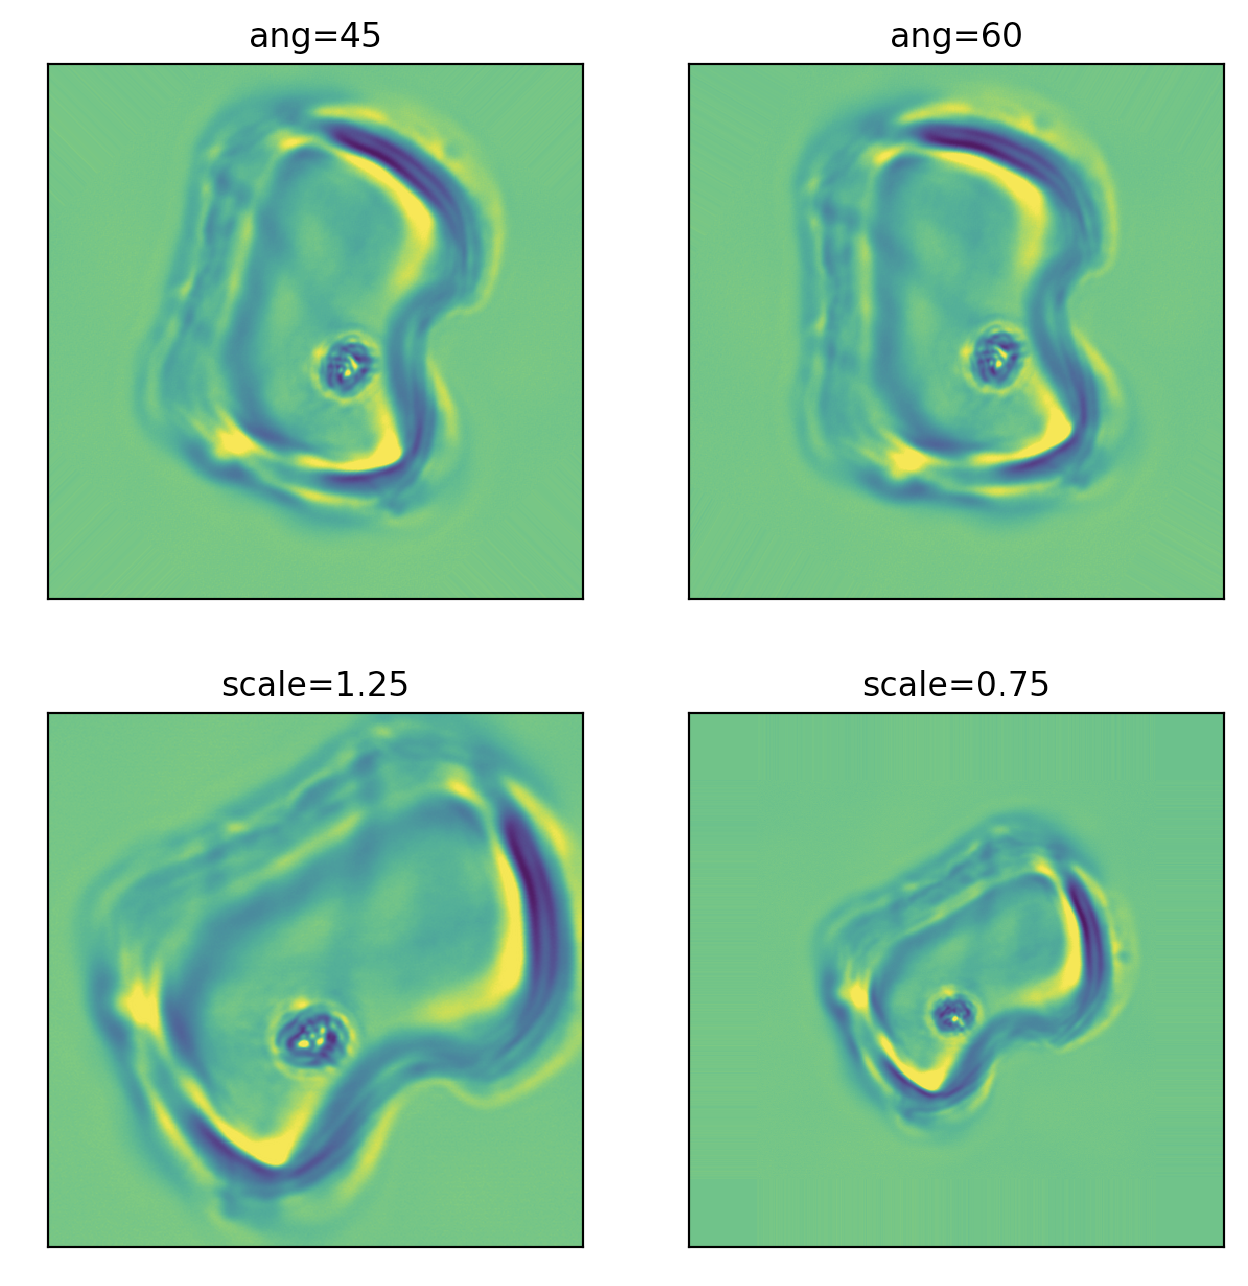
\includegraphics[width=0.5\textwidth]{rotations}
	\caption{Rotated and scaled data generated from a data sample}
	\label{fig:rotated}
\end{figure}

\section{Data Preprocessing}

As mentioned, the dataset only contains 889 data samples, resulting in as little as one example in several classes. This motivated See Figure \ref{fig:rotated} for an example of our synthetic data.

\section{Baseline Models \& Result}

Our baseline models include a linear classifier and a CNN model. In this section, we use $\mathbf{X}$ and $\mathbf{y}$ to refer to our training input and output, where each ${x}_i^T\in \mathbf{X}$ is a vector representing a image and each ${y_i}\in \mathbf{y}$ is the label of that image. Depending on the training objective, the label $y_i$ is an integer either between 0-7 (for predicting both family and sub-family) or 0-1 (for family only). We use $\mathbf{p}$ to represent predictions made by our classifier. Our model is implemented using Tensorflow v1.4.

Each raw image stack (shaped 256 * 512 * 512) is compressed into one single image (512 * 512) by mean-pooling, and then uniformly resized into 128 * 128 sized images.

\paragraph{Linear Model}

Our linear model predicts the label using linear transformation, as follows

$$\mathit{logits} = \mathbf{X} \mathbf{W} + \mathbf{b}$$
$$\mathbf{p} = \arg\max(\mathit{logits})$$


The training objective is to minimize the cross entropy loss (with L1 regularization):

$$\mathit{loss} = -\sum\limits_{i} y_i\log(\mathit{softmax}(\mathit{logits})) + \lambda \|\mathbf{W}\|_1$$

\paragraph{CNN Model}

Our CNN model is a two layer convolution network. The first layer consists of 32 filters and the second with 64 filters, both using max-pooling with stride 2 and kernel size 2.

The output from the second layers is implemented with dropout 0.4 to avoid over-fitting due to the small amount of data, and then the result is sent to a fully connected layer for decoding, which is the same as the one in the linear model.

\medskip

Both of our models are trained using Adagrad optimizer with learning rate 0.1 and trained 40 epoches.
Our result shows that the CNN model achieves 80.5\% validation accuracy on family classification and 34.7\% 7-class classification, while the linear model achieves 89.4\% in the 2-classes task and 57.1\% in the 7-class task.


\section{Follow-up Plans}

\paragraph{Transfer learning} One problem of the dataset is that we have a very small set of the data (889 image stacks), and CNN model does not benefit from its expressiveness. Our plan is to include a synthetic dataset to initialize our model together with phytolith datasets from other sources (Missouri Phytolith Database~\footnote{http://phytolith.missouri.edu/}, and Phytcore dataset~\footnote{http://www.phytcore.org/phytolith/}).

\paragraph{Utilizing 3D information from image stacks}

In order to use common image recognition techniques (such as convolutional neural networks) to analyze the data, some simple methods to reduce the dimensionality of the data exist, such as taking the mean, minimum, or maximum along the depth axis. However, this discards information. 

We intend to make better use of the 3D information present in the raw data by developing a neural network architecture specifically for classifying 3D voxels\cite{DBLP:conf/iros/MaturanaS15,brock2016generative}. Due to the relative scarcity of data for a deep learning approach, we have decided to augment our dataset with synthetic data so that our model can better learn the relationship between shapes and their image stack representations. For example, we might take a deformable part model approach by learning to recognize certain primitives shapes that comprise the 3D structures. To this end, we have developed a framework for generating synthetic confocal microscope data from basic 3D shapes, creating image stacks with the objects oriented randomly. It is also important to incorporate the optical artifacts inherent to the measurement technique, which we have done by convolving the sharp 3D volumes with a depth-axis aligned conic filter. Topics of future investigation will therefore involve choosing a set of features with reasonable coverage, finding a neural network architecture that is suited to the associated recognition tasks, and assessing the performance of a classification method using these features.

\bibliography{milestone}
\bibliographystyle{plain}
\end{document}